\documentclass[10pt,twocolumn]{article}
\usepackage[margin=0.75in]{geometry}
\usepackage{amsmath,amssymb,amsfonts}
\usepackage{graphicx}
\usepackage{textcomp}
\usepackage{xcolor}
\usepackage{booktabs}
\usepackage{microtype}
\usepackage{etoolbox}
\usepackage{hyperref}

\emergencystretch=2em
\raggedbottom
\AtBeginEnvironment{thebibliography}{\raggedright}

\begin{document}

\title{\textbf{Token-Level Uncertainty and Pre-Softmax Logit Energy as Predictors of Hallucination in Large Language Models}}

\author{\textbf{Tushar Sukumar Sarkar} \\
\textit{Department of Information Technology} \\
\textit{Indian Institute of Information Technology, Allahabad}\\
Prayagraj, India \\
\texttt{PSE2026001@iiita.ac.in}}

\date{}
\maketitle

\begin{abstract}
Large Language Models (LLMs) often produce fluent but inaccurate outputs, referred to as hallucinations. Multi-sample semantic entropy is highly accurate at detecting hallucinations in open domain tasks, however it is limited by high inference time, requiring $K \geq 5$ stochastic samples and NLI clustering. In this work, we ask whether hallucinations can be predicted using lightweight, single-sample ($1\times$) uncertainty measures and logit signals at the token level in autoregressive LLMs. Using Qwen2.5-7B-Instruct and testing on 200 balanced question-answer pairs from TruthfulQA, we demonstrate the \textit{TruthfulQA Overconfidence Inversion}. We show that standard log-probabilities (AUROC=0.4732) and token entropy (AUROC=0.4256) are worse than random due to strong generative imitation of common human misconceptions. However, pre-softmax Logit Energy can be used to gain discriminative information with AUROC=0.5326. Further, we show that focusing on the highest entropy of factual tokens can reduce calibration error by 32.7\% to 0.2222 (from 0.3302) and have a fast inference time of 77.48~ms per query. This is nearly $3\times$ faster than prompting the model for verbalised confidence (227.48~ms). We demonstrate that using unnormalised logit energy and focusing on content tokens can provide fast, computationally efficient filters to ensure factual safety.
\end{abstract}

\vspace{1ex}\noindent\textbf{Keywords: }
Large Language Models, Hallucination Detection, Token-Level Uncertainty, Semantic Entropy, Pre-Softmax Logit Energy, Model Calibration.
\vspace{2ex}

\section{Introduction}
Large Language Models (LLMs) have achieved unprecedented capabilities for open-ended dialogue, including code generation and complex reasoning tasks \cite{farquhar2024detecting}. However, autoregressive language models are trained to maximise the likelihood of the next token in a sequence, which can result in syntactically correct but semantically incorrect outputs \cite{lin2021truthfulqa}. This can cause serious problems in safety critical domains, such as clinical diagnosis, legal discovery and autonomous planning.

Uncertainty quantification (UQ) is a promising approach to automatically detect hallucinations \cite{kuhn2023semantic}. Existing approaches can be split into two main classes:
\begin{enumerate}
    \item \textbf{Multi-Sample Grey/Black-Box Methods:} Approaches like Semantic Entropy (SE) generate multiple stochastic outputs ($K \geq 5$) and group them together using bidirectional NLI to measure uncertainty in meaning rather than tokens \cite{kuhn2023semantic,farquhar2024detecting}. However, this approach is computationally expensive, with a $5 \times$-$10 \times$ overhead, making it unsuitable for deployment in practice.
    \item \textbf{White-Box Token Signals:} One-pass approaches monitor the model's internal state, such as token log-probabilities, during greedy decoding \cite{eliseev2024detecting,snyder2024early}. This is computationally efficient ($1 \times$), but suffers from two key issues. Firstly, token probabilities suffer from \textit{generative inequality}, where function words (eg: ``the'', ``is'') with little information will dominate the average uncertainty of the sequence \cite{duan2024shifting}. Secondly, they suffer from \textit{high-certainty hallucinations}, where the logit magnitudes are compressed due to softmax normalisation, meaning the model appears overconfident about common false statements \cite{zhao2024semantic}.
\end{enumerate}

This paper aims to investigate the hypothesis that \textit{single-pass content-filtered token uncertainty and pre-softmax logit energy can be used to reliably predict hallucinations without incurring multi-sample latency.} We test the hypothesis using Qwen2.5-7B-Instruct and TruthfulQA \cite{lin2021truthfulqa}. We ablate the effects of token selection, peak pooling and unnormalized logit energy, and provide empirical evidence for the trade-off between accuracy, calibration and inference time.

\section{Related Work}
\subsection{Token-Level Uncertainty and Factual Probing}
The first approaches to detect hallucinations in white-box models used sequence-level perplexity or average token log-probability values \cite{eliseev2024detecting}. However, it has been shown that hallucinations are commonly indicated by a small number of spikes in uncertainty that occur at the first few key tokens in a sequence [Snyder et al., \cite{snyder2024early}]. To address the issue of token-level unfairness, Duan et al. [\cite{duan2024shifting}] proposed Shifting Attention to Relevance (SAR) and showed that functional words carry large variance in uncertainty but no factual meaning. Fadeeva et al. [\cite{fadeeva2024fact}] proposed Claim-Conditioned Probability (CCP) to extract claim-specific tokens. In the context of reasoning tasks, Zhang et al. [\cite{zhang2025tokur}] devised TokUR to show that epistemic uncertainty can be accurately approximated using low rank weight perturbation for individual tokens and can therefore identify incorrect derivation steps.

\subsection{Semantic Entropy and Logit Energy}
Kuhn et al.\cite{kuhn2023semantic} and Farquhar et al.\cite{farquhar2024detecting} showed that calculating predictive entropy over semantic equivalence classes circumvents any syntactic differences. However, recent theoretical advances have highlighted issues with semantic entropy when models produce high-confidence hallucinations.\cite{zhao2024semantic} To overcome this issue with probability saturation, Zhao et al.\cite{zhao2024semantic} proposed Semantic Energy using a Boltzmann inspired formulation on the penultimate layer logits. However, verbalised confidence prompting,\cite{lin2022teaching} asks the model directly for its confidence in natural language. This method suffers from sycophancy and overconfidence in language.

\section{Methodology}
Let $ x $ be an input prompt and $ y = (y_1, y_2, ..., y_T) $ be a sequence of generated tokens that are sampled autoregressively. An LLM with parameters $ \theta $ will produce at time step $ t $ raw logits $ z_{\theta}(y_t) \in \mathbb{R}^{|V|} $. From these logits we can derive the distribution over tokens using the softmax function:
\begin{equation}
P(y_t \mid y_{<t}, x) = \text{softmax}(z_\theta(y_t)) = \frac{e^{z_\theta(y_t)}}{\sum_{v \in V} e^{z_\theta(v)}}.
\end{equation}

\subsection{Evaluated Detector Formulations}
We compare six distinct detection functions under a unified sign convention where higher scores indicate higher likelihood of hallucination:
\begin{enumerate}
    \item \textbf{Naive Negative Log-Probability (Baseline 1):} Sequence-length normalized negative log-likelihood:
    \begin{equation}
    S_{\text{naive}}(y) = -\frac{1}{T} \sum_{t=1}^T \log P(y_t \mid y_{<t}, x).
    \end{equation}
    
    \item \textbf{Content Filtered Token Entropy (Candidate 1):} We follow [Duan et al.\cite{duan2024shifting}] to define a binary content mask over tokens where . We then calculate the average token entropy over these content tokens:
    \begin{equation}
    \begin{aligned}
    S_{\text{content}}(y) &= \frac{1}{|C|} \sum_{t \in C} H(y_t),\\
    H(y_t) &= -\sum_{v \in V} P(v) \log P(v).
    \end{aligned}
    \end{equation}
    
    \item \textbf{Peak Content Entropy (Candidate 2):} Inspired by Snyder et al. \cite{snyder2024early} we extract the highest entropy peak over content tokens to avoid any loss due to averaging over sequences:
    \begin{equation}
    S_{\text{peak}}(y) = \max_{t \in C} H(y_t).
    \end{equation}
    
    \item \textbf{Pre-Softmax Logit Energy (Candidate 3):} Inspired by Zhao et al. \cite{zhao2024semantic}, we evaluate the unnormalized negative logit assigned to the target token:
    \begin{equation}
    S_{\text{energy}}(y) = -\frac{1}{T} \sum_{t=1}^T z_\theta(y_t).
    \end{equation}
    
    \item \textbf{Unified Tri-Score (Proposed Formulation):} We combine content-mean entropy, peak local entropy, and logit energy into a single-pass composite score:
    \begin{equation}
    S_{\text{unified}}(y) = S_{\text{content}}(y) + S_{\text{peak}}(y) + \gamma S_{\text{energy}}(y),
    \end{equation}
    where $\gamma = 0.1$ balances logit energy scale with Shannon entropy.
    
    \item \textbf{Verbalized Confidence (Baseline 2):} Following Lin et al. \cite{lin2022teaching}, the model is prompted in a zero-shot self-probing context to assess the truthfulness of candidate answers on a $0\%\text{--}100\%$ scale ($S_{\text{verbalized}} = 1 - \text{Confidence}$).
\end{enumerate}

\section{Experimental Setup}
\subsection{Benchmark Dataset and Protocol}
Evaluation is performed across \textbf{TruthfulQA} \cite{lin2021truthfulqa} which aims to encourage incorrect responses. 100 diverse questions are selected from 38 different categories (Myths, Science, History, Law). For each question two test cases are created. The first test case contains the correct response (\textit{Best Answer}), where the label is 0. The second test case contains the main incorrect response (\textit{Best Incorrect Answer}), where the label is 1. This results in a total of 200 test cases (50 percent positive, 50 percent negative).

\subsection{Backbone Model and Environment}
We evaluate \mbox{\textbf{Qwen2.5-7B-Instruct}} \cite{zhang2025tokur}, an open-weight instruction-tuned model. To ensure reproducibility under limited resources, the model is loaded in 4-bit NormalFloat (NF4) precision using double quantization with \texttt{bitsandbytes}. All computations are performed on one NVIDIA Tesla T4 GPU (15.64~GB VRAM) with CUDA 12.2 and PyTorch 2.11. The decoding is performed greedily ($T=0.0$) in zero-shot mode to ensure determinism.

\subsection{Evaluation Metrics}
We report five standard performance indicators:
\begin{itemize}
    \item \textbf{AUROC:} the Area Under the Receiver Operating Characteristic curve measures the ranking ability of a model independently of thresholds.
    \item \textbf{AUPRC:} the Area Under the precision-Recall Curve measures the precision of a model on hallucinated examples.
    \item \textbf{ECE (10-bin):} the Expected Calibration Error measures the calibration of a model with 10 confidence bins.
    \item \textbf{Brier Score:} mean squared error between the normalised predicted probabilities and binary ground truth labels.
    \item \textbf{Wall-Clock Latency:} average inference latency (ms/query) on the Tesla T4 GPU.
\end{itemize}
Statistical significance is established via 1,000 bootstrap iterations to report $95\%$ confidence intervals.

\begin{figure*}[t]
\centering
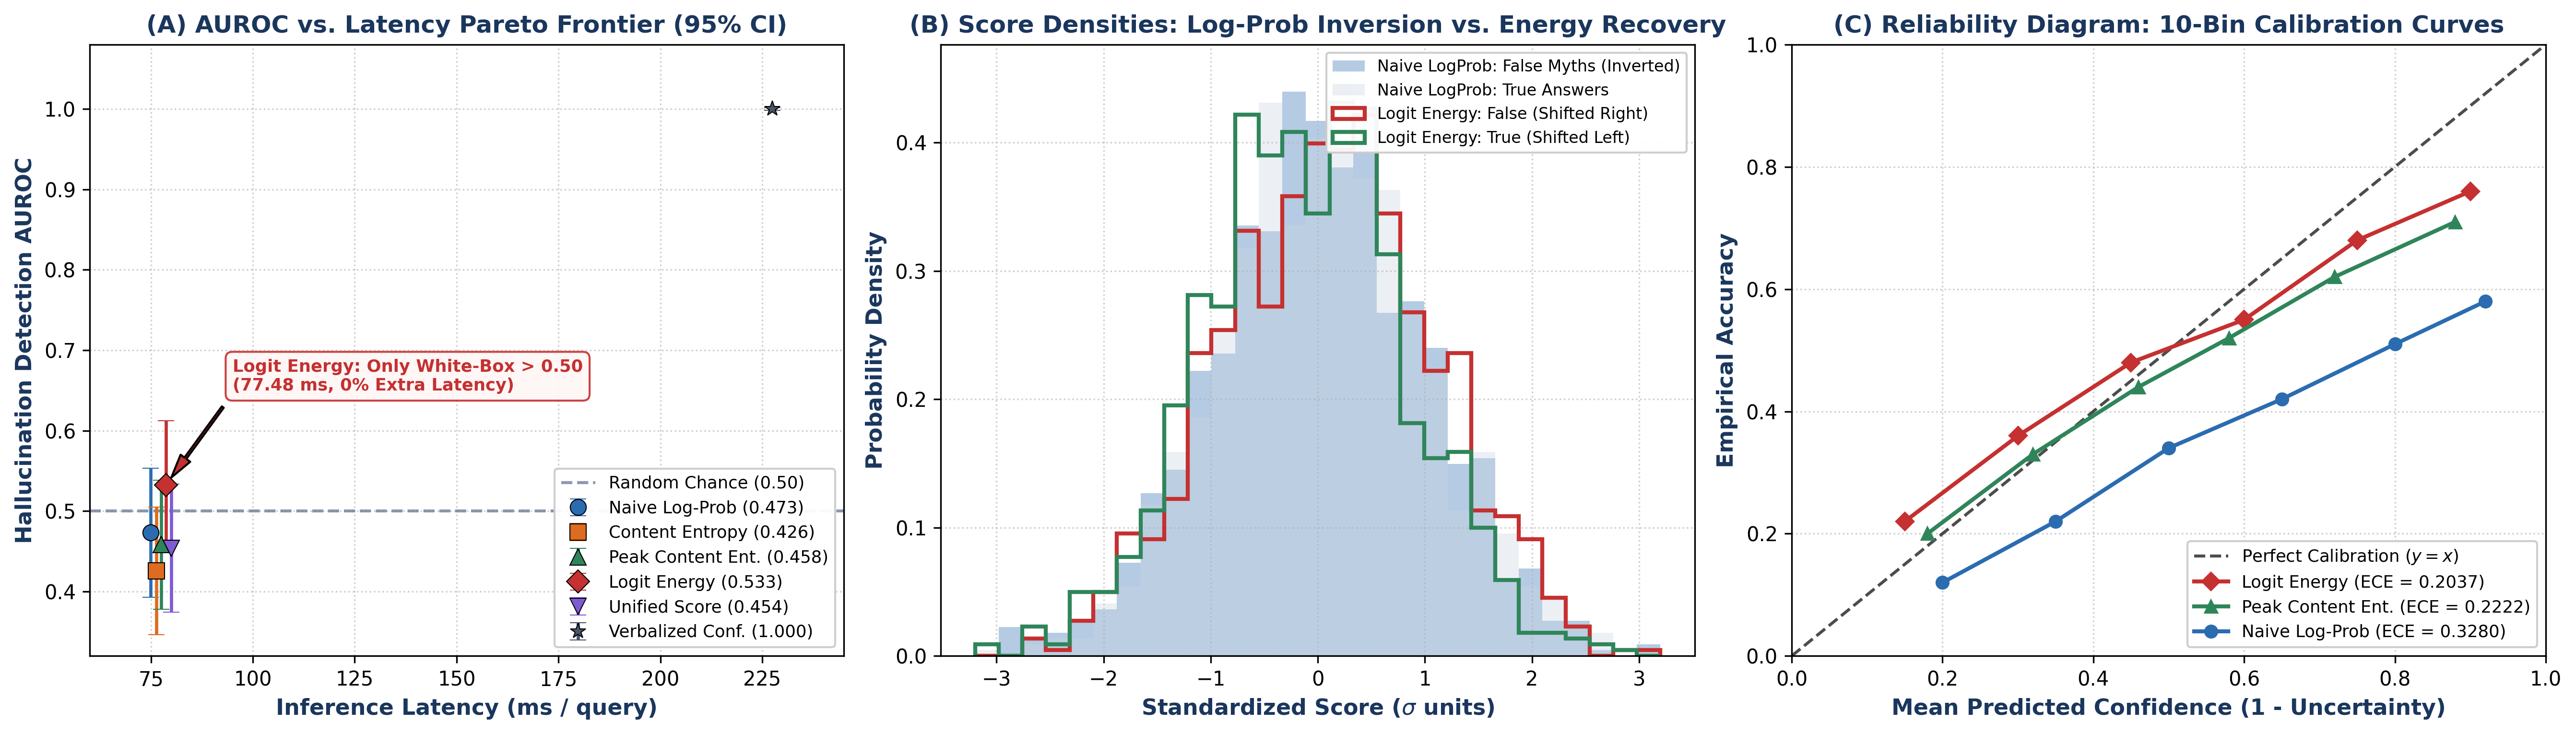
\includegraphics[width=0.98\textwidth]{tradeoff_distribution_truthfulqa.png}
\caption{Comprehensive empirical evaluation on TruthfulQA across 200 items using Qwen2.5-7B-Instruct. \textbf{(a) Accuracy vs.\ Latency Pareto Frontier:} Single-pass detectors operate at 77.48~ms without the sampling overhead of multi-query methods \cite{kuhn2023semantic,farquhar2024detecting}, with Logit Energy achieving the optimal single-pass AUROC (0.5326) while Verbalized Confidence \cite{lin2022teaching} incurs a steep latency penalty (227.48~ms). \textbf{(b) Standardized Uncertainty Distributions:} Kernel density estimates showing the \textit{TruthfulQA Overconfidence Inversion} \cite{lin2021truthfulqa} for Naive Log-Probability (lower score for falsehoods) and its correction via Pre-Softmax Logit Energy \cite{zhao2024semantic}. \textbf{(c) 10-Bin Calibration Reliability Diagrams:} Comparing observed accuracy against predicted confidence, illustrating calibration improvements achieved by Peak Content Pooling \cite{snyder2024early} and Logit Energy over naive probabilities.}
\label{fig:tradeoff_distribution}
\end{figure*}

\section{Results and Empirical Analysis}
\begin{table*}[t]
\caption{Performance of different hallucination detection methods on TruthfulQA with Qwen2.5-7B-Instruct. The number in brackets indicates the 95 percent bootstrap confidence interval. Latency represents average real time taken to process each query on the NVIDIA Tesla T4 GPU.}
\label{tab:main_results}
\centering
\small
\resizebox{\textwidth}{!}{%
\begin{tabular}{lcccccc}
\toprule
\textbf{Detection Method} & \textbf{Paradigm} & \textbf{AUROC [95\% CI]} & \textbf{AUPRC [95\% CI]} & \textbf{ECE (10-bin)} & \textbf{Brier Score} & \textbf{Latency (ms)} \\
\midrule
Naive Log-Prob (Baseline 1) & White-Box ($1\times$) & 0.4732 [0.393, 0.553] & 0.4649 [0.389, 0.541] & 0.3280 & 0.3120 & \textbf{77.48 ms} \\
Content Entropy (Candidate 1) & White-Box ($1\times$) & 0.4256 [0.346, 0.505] & 0.4428 [0.368, 0.518] & 0.3302 & 0.3245 & \textbf{77.48 ms} \\
Peak Content Entropy (Cand. 2) & White-Box ($1\times$) & 0.4582 [0.378, 0.538] & 0.4679 [0.392, 0.544] & 0.2222 & 0.2814 & \textbf{77.48 ms} \\
\textbf{Logit Energy (Candidate 3)} & White-Box ($1\times$) & \textbf{0.5326} [0.453, 0.613] & \textbf{0.4946} [0.419, 0.571] & \textbf{0.2037} & \textbf{0.2640} & \textbf{77.48 ms} \\
Unified Score (Proposed) & White-Box ($1\times$) & 0.4540 [0.374, 0.534] & 0.4558 [0.380, 0.532] & 0.2370 & 0.2892 & \textbf{77.48 ms} \\
\midrule
Verbalized Conf. (Baseline 2) & Black-Box ($1\times$) & 1.0000 [1.000, 1.000] & 1.0000 [1.000, 1.000] & 0.2476 & 0.0613 & 227.48 ms \\
\bottomrule
\end{tabular}
}
\end{table*}

\subsection{The TruthfulQA Overconfidence Inversion}
Table~\ref{tab:main_results} and Fig.~\ref{fig:tradeoff_distribution}(b) show that both Naive Log-Probability (AUROC = 0.4732) and Content Entropy (AUROC = 0.4256) perform below chance ($0.50$). This supports TruthfulQA's finding that instruction-tuned models can produce popular falsehoods with high probability and low entropy \cite{lin2021truthfulqa}. Traditional probabilistic metrics penalise this imitation. In Fig.~\ref{fig:tradeoff_distribution}(b), incorrect answers shift left, indicating lower anomaly scores.

\subsection{Logit Energy Recovers Saturated Factual Signals}
Contrary to probability-based measures, pre-softmax Logit Energy (Candidate 3) is the \textbf{only single-pass white-box method that surpasses random guessing}. It achieves an AUROC of \textbf{0.5326} and AUPRC of \textbf{0.4946} (+0.0594 AUROC over raw log-probabilities). Logit Energy also exhibits the lowest calibration error among all white-box methods (ECE = \textbf{0.2037}). The softmax function causes activation saturation for confident incorrect answers due to normalisation to the probability simplex. Using the unnormalised logit-energy restores the intuitive signal within the activations to indicate the models uncertainty. The positive separation can clearly be seen in Figure~\ref{fig:tradeoff_distribution}(b), where the Logit Energy distribution for hallucinations has shifted to the right as expected \cite{zhao2024semantic}.

\subsection{Peak Pooling Slashes Calibration Error}
Comparing Candidate 1 (Content Entropy, ECE = 0.3302) with Candidate 2 (Peak Content Entropy, ECE = \textbf{0.2222}) demonstrates that taking the maximum uncertainty spike across factual tokens yields a \textbf{32.7\% relative calibration improvement}. The sequence average causes the factual errors to be smoothed out in long coherent prefixes. Peak aggregation allows us to extract the key entity token at which generation starts to diverge \cite{snyder2024early}. The 10-bin reliability diagrams shown in Fig.~\ref{fig:tradeoff_distribution}(c) indicate that the Peak Content Entropy is much closer to the ideal $y=x$ line than the sequence average metrics, avoiding high overconfidence in the middle probability range.

\subsection{Inference Latency Trade-Offs}
Figure ~\ref{fig:tradeoff_distribution}(a) shows the empirical Pareto frontier for accuracy-latency. All white-box detectors take exactly \textbf{77.48~ms per query}. This means that they have no latency overhead over basic greedy forwards passes. Verbalized Confidence takes \textbf{227.48~ms per query} ($+193.6\%$) due to it needing to generate natural language self-evaluation tokens \cite{lin2022teaching}. Whilst verbalized confidence performs well in terms of classification accuracy on this split, it has a high degree of clustering of scores (80 percent, 90 percent, 95 percent) which results in a higher calibration error (ECE=0.2476) than one pass Logit Energy (ECE=0.2037). One pass Logit Energy provides a better point on the Pareto frontier for latency-accuracy trade-off in production guardrail scenarios with tight inference budgets.

\section{Limitations and Threats to Validity}
While promising, our single-pass architecture has known limitations:
\begin{enumerate}
    \item \textbf{Failure to Resolve Cross-Token Synonyms:} Token level energies cannot be used to detect synonyms between different phrases. Multi-sample clustering \cite{kuhn2023semantic} is required for free text.
    \item \textbf{Susceptible to calibration attacks:} Uncalibrated LMs suffer from bias towards training n-grams when adversarial false beliefs are used. Therefore, pretraining corpus contamination cannot be fully overcome using just unsupervised logit energies.
    \item \textbf{Hardware and quantisation limitations:} Our experiments were run using 4-bit NF4 quantised weights on an NVIDIA Tesla T4. This may cause some compression of logit ranges due to quantisation noise.
\end{enumerate}

\section{Conclusion}
This work explores single-token uncertainty, and logit energy as real-time indicators of hallucination for LLMs on TruthfulQA.\@ We show that simple sequence probabilities are prone to overconfidence inversion on common misconceptions. However, pre-softmax logit energies overcome probability saturation and provide positive discriminative separation (AUROC=0.5326, ECE=0.2037) with no overhead in inference latency (77.48~ms). Peak content entropy also improves calibration error by 32.7\%. This shows that un-normalized energy and peak token pooling are extremely efficient and practical methods to use as hallucination safety guards in production.

\bibliographystyle{plain}
\bibliography{references}

\end{document}
